\subsection{DIANE – Dynamic IoT Application Deployment}
\textit{DIANE} merupakan penelitian lanjutan dari LEONORE yang telah dijelaskan pada bagian \ref{subsec:leonore}. DIANE adalah sebuah sistem ataupun \textit{framework} yang dapat menghasilkan topologi \textit{deployment} secara dinamis yang dioptimalkan untuk aplikasi IoT serta disesuaikan dengan infrastruktur terkait.

Berbeda dengan LEONORE, DIANE tidak menggunakan \textit{application package}, melainkan menggunakan model deklaratif berbasis \textit{resource} dari \textit{aplikasi} yang dibuat. Pendekatan ini memungkinkan penyediaan komponen aplikasi yang fleksibel pada infrastruktur \textit{cloud} serta \textit{gateway} IoT \parencite{vogler2015diane}. DIANE menggunakan \textit{Methodology for Architecture and Deployment of Cloud Application Topologie} (MADCAT) untuk mendefinisikan komponen yang digunakan. Pada metode ini, terdapat dua unit yang menjadi komponen penting pada sistem, yaitu \textit{Technical Unit}(TU) serta \textit{Deployment Unit}(DU) \parencite{madcat}. TU berikatan dengan aplikasi yang ingin dibuat sehingga satu \textit{TU} dapat memiliki satu atau lebih \textit{DU} yang mendefinisikan proses \textit{deployment} yang dibuat. Ilustrasi TU dan DU dapat dilihat pada gambar \ref{fig:diane-tu} dan \ref{fig:diane-du}.

\begin{figure}[ht]
  \centering
  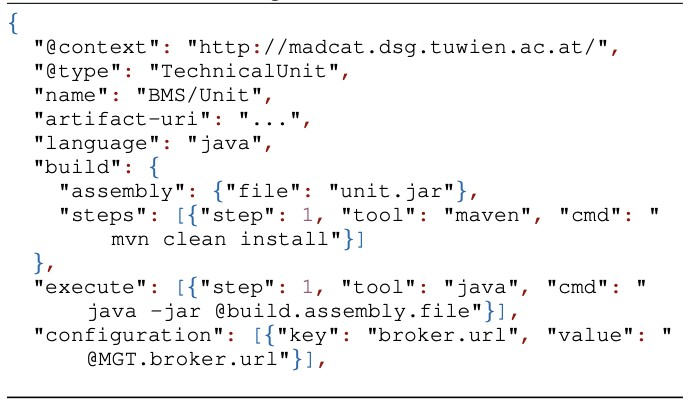
\includegraphics[width=0.8\textwidth]{resources/chapter-2/diane-technical-unit.jpg}
  \caption{\textit{Technical Unit} DIANE \parencite{vogler2015diane}}
  \label{fig:diane-tu}
\end{figure}

\begin{figure}[ht]
  \centering
  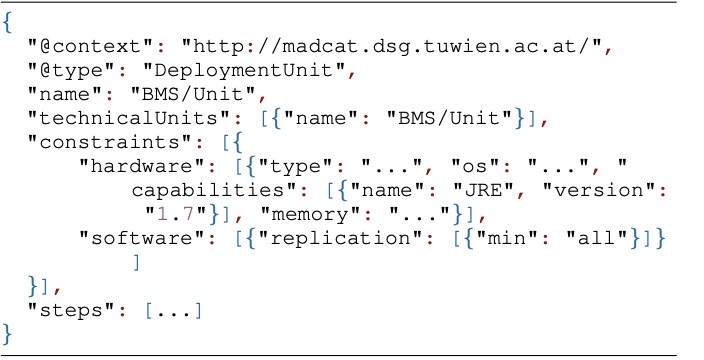
\includegraphics[width=0.8\textwidth]{resources/chapter-2/diane-deployment-unit.jpg}
  \caption{\textit{Deployment Unit} DIANE \parencite{vogler2015diane}}
  \label{fig:diane-du}
\end{figure}

DIANE memiliki arsitektur yang terdiri dari \textit{Deployment Registry}, \textit{Deployment Handler}, \textit{Artifact Management}, \textit{Deployment Generator}, \textit{Dependency Management}, dan \textit{Constraint Handler}. Setelah seluruh proses dilewati, DIANE akan berinteraksi dengan \textit{Service API} untuk melakukan \textit{provisioning} dengan LEONORE. Ilustrasi arsitektur DIANE dapat dilihat pada gambar \ref{fig:diane-arch}.

\begin{figure}[ht]
  \centering
  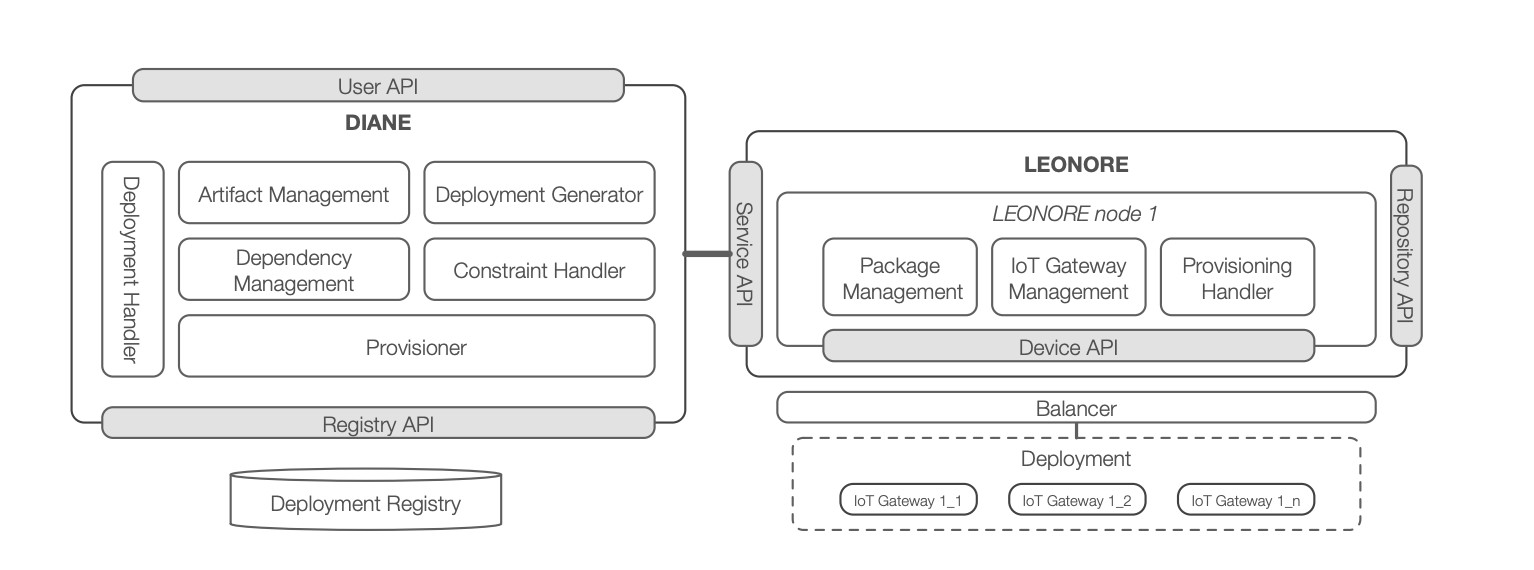
\includegraphics[width=0.8\textwidth]{resources/chapter-2/diane-architecture.jpg}
  \caption{Arsitektur DIANE \parencite{vogler2015diane}}
  \label{fig:diane-arch}
\end{figure}